\subsection{Resistive Wall Impedance}
\label{sec:res_wall_imp}

The resistive wall impedance is an impedance generated due to the finite conductivity of the material of the beam pipe wall. This can have a number of regimes dependent on whether the skin depth of the material $\delta \left( \omega \right) = \sqrt{\frac{2}{\mu_{0} \mu_{r} \sigma \omega}}$ ($\mu_{0}$ being the permeability of free space, $\mu_{r}$ the relative permeability of the material, $\sigma$ the conductivity of the wall material) is much smaller than the thickness of the beam pipe wall \cite{Chao:PhysColEff}, comparable to the thickness of the beam pipe wall \cite{Roncarolo:ColImpMeas, Metral:ResWallWideFreq} or much larger than the thickness of the beam pipe wall \cite{Tsutsui:ferrKickLong, Biancacci:MMFiniteInsert}, in addition to the pipe radius and the thickness of the pipe wall (such as the case of an a pipe wall of infinite thickness). In this instance, $\sigma$ is the conductivity of wall material. It can also be shown that the shape of the beam pipe cross section also plays a significant role in defining the impedance \cite{Mounet:Axisymmetric, Mounet:Flat}.

Here we shall not attempt a comprehensive summary of the various resistive wall impedance models, but simply give an introduction to the Tsutsui formalism to give a sense of how changing the wall conductivity affects the resistive wall impedance. A considerably more detailed overview of this derivation can be found in \cite{Tsutsui:ferrKickLong, Tsutsui:DipoleKicker}. Consider a two parallel plates of a resistive material, as shown in Fig.~\ref{fig:res_wall_diagram}, between which moves a source particle of charge $q_{1}$ moving with velocity $\mathbf{v} = \beta c \mathbf{\hat{z}}$. In this case it shall be assumed that $\beta = 1$.

\begin{figure}
\begin{center}
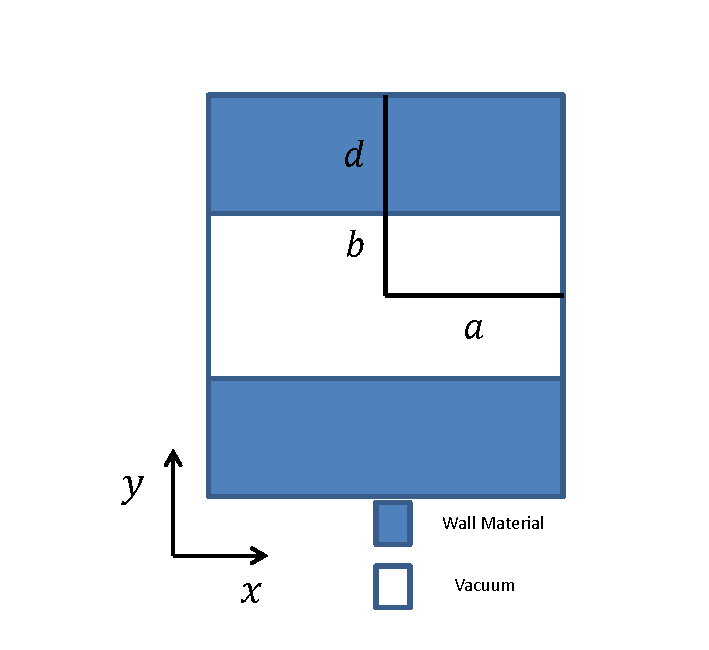
\includegraphics[width=0.6\textwidth]{Wakefields_and_Impedances/figures/reWallGeo.pdf}
\end{center}
\caption{The geometry of the Tsutsui resistive wall formalism.}
\label{fig:res_wall_diagram}
\end{figure}

The longitudinal and dipolar impedances for this model can be seen in Fig.~\ref{fig:resWallImpComp} for a comparison between two sample materials. It can be seen that for the given frequency range there are two regimes for both the longitudinal and transverse impedance (although the difference more pronounced for the transverse impedance). For high frequencies, the classical thick wall formalism (as in \cite{Chao:PhysColEff}) applies, as the skin depth of the material is much smaller than the beam pipe aperture and the layer's thickness. Susequently this formalism would predict a greater impedance at lower frequencies, as it gives $Z_{\perp} \propto \omega^{-1/2}$. At lower frequencies however this is not seen to be the case. This is due to the following reasons:

\begin{enumerate}
\item{At high frequencies the beam induced current effectively flows on the surface of the material, thus the distance between the beam image current and the witness particle is constant at value $b$. Thus the transverse impedance seen is determined by the change in skin depth $\delta$ which is proportional to $\omega^{-1/2}$}
\item{At low frequencies the beam image current effectively flows some distance inside the wall material, greater than $b$. This increases the distance between the beam image current and the witness particle, thus decreased the force seen by the witness particle. This causes the transverse impedance to become linear with respect to $\omega$. It is important to note this mechanism, as it indicates that this phenomena occurs at a "low" frequency for any thickness of wall material, even for a wall of infinite thickness.}
\item{The transition region occurs when these two phenomena become of similar magnitude. The frequency at which the real component of the transverse impedance reaches it's maximum can be shown to be proportional to $1/(\sigma b^{2})$.}
\end{enumerate}

\begin{figure}
\subfigure[]{
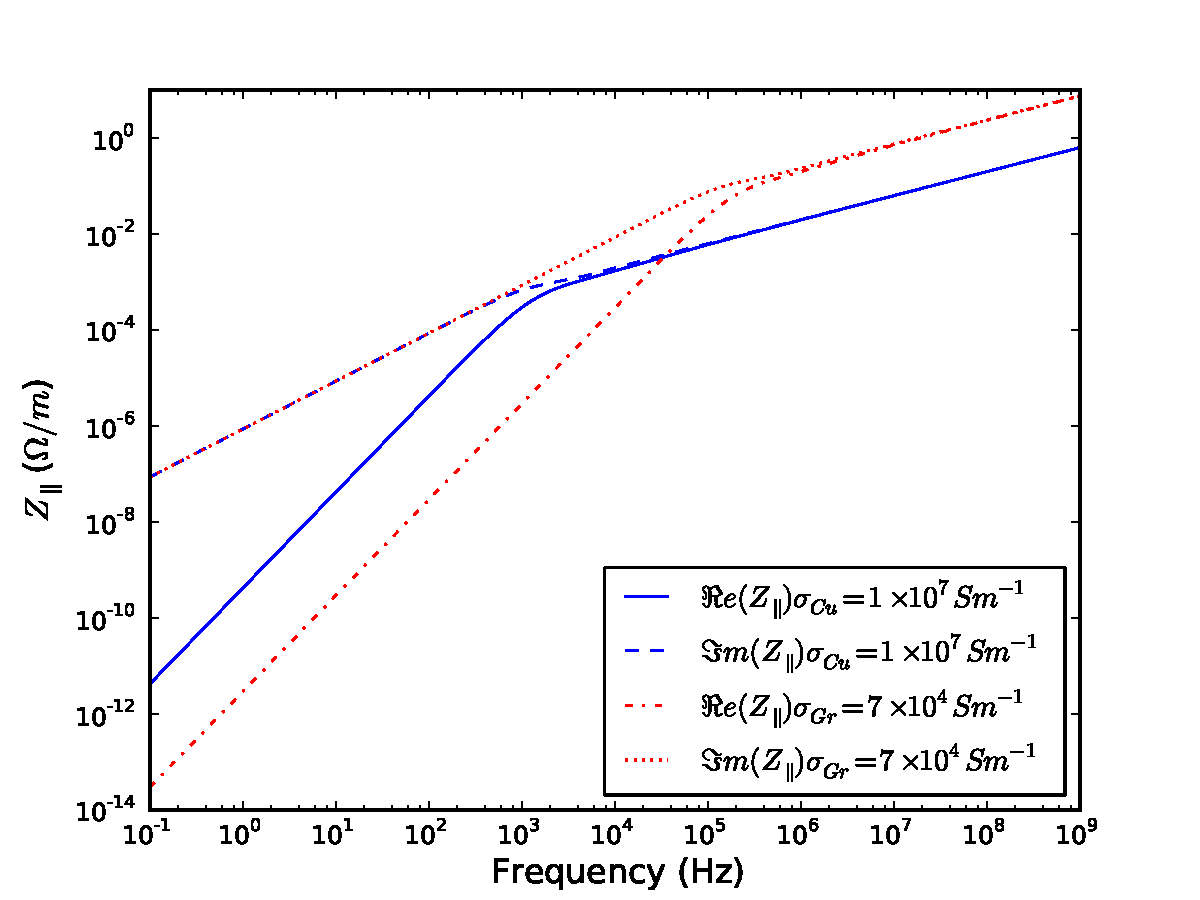
\includegraphics[width=0.5\textwidth]{Wakefields_and_Impedances/figures/resWallTsutsuiLong.pdf}
\label{fig:reswalllong}
}
\subfigure[]{
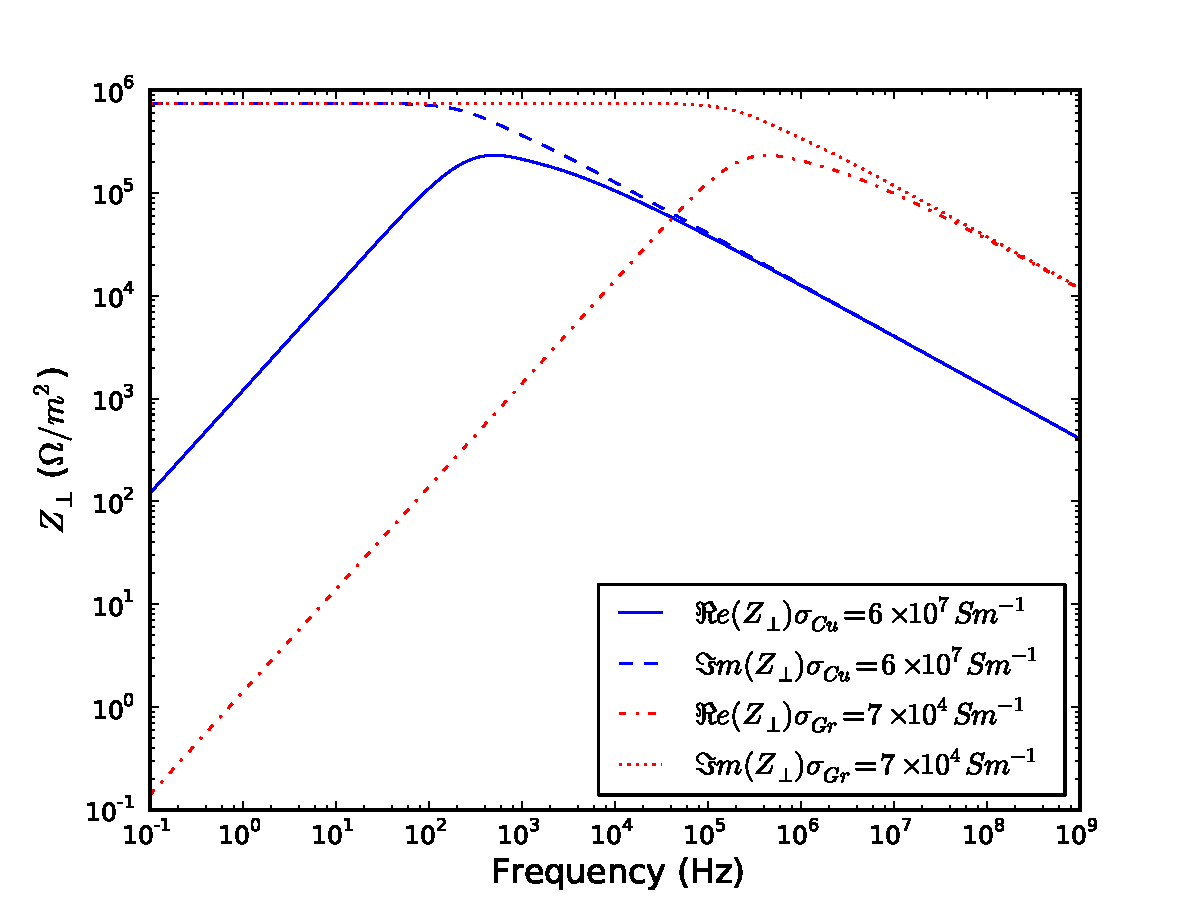
\includegraphics[width=0.5\textwidth]{Wakefields_and_Impedances/figures/resWallTsutsuiTrans.pdf}
\label{fig:reswalltrans}
}

\caption{Examples of the longitudinal \ref{fig:reswalllong} and transverse \ref{fig:reswalltrans} resistive wall impedance per unit length of a beam pipe of radius $a = 2cm$ made of both copper ($\sigma = 1 \times 10^{7} S m^{-1}$) and graphite ($\sigma = 7 \times 10^{4} S m^{-1}$).}
\label{fig:resWallImpComp}
\end{figure}

